% !TEX TS-program = pdflatex
% !TEX encoding = UTF-8 Unicode

% This is a simple template for a LaTeX document using the "article" class.
% See "book", "report", "letter" for other types of document.

\documentclass[11pt]{article} % use larger type; default would be 10pt

\usepackage[utf8]{inputenc} % set input encoding (not needed with XeLaTeX)

%%% Examples of Article customizations
% These packages are optional, depending whether you want the features they provide.
% See the LaTeX Companion or other references for full information.

%%% PAGE DIMENSIONS
\usepackage{geometry} % to change the page dimensions
\geometry{a4paper} % or letterpaper (US) or a5paper or....
\geometry{margin=1in} % for example, change the margins to 2 inches all round
% \geometry{landscape} % set up the page for landscape
%   read geometry.pdf for detailed page layout information

\usepackage{graphicx} % support the \includegraphics command and options

% \usepackage[parfill]{parskip} % Activate to begin paragraphs with an empty line rather than an indent
\usepackage{amssymb}
\usepackage{amsmath}
%%% PACKAGES
\usepackage{booktabs} % for much better looking tables
\usepackage{array} % for better arrays (eg matrices) in maths
\usepackage{paralist} % very flexible & customisable lists (eg. enumerate/itemize, etc.)
\usepackage{verbatim} % adds environment for commenting out blocks of text & for better verbatim
\usepackage{subfig} % make it possible to include more than one captioned figure/table in a single float
% These packages are all incorporated in the memoir class to one degree or another...

%%% HEADERS & FOOTERS
\usepackage{fancyhdr} % This should be set AFTER setting up the page geometry
\pagestyle{fancy} % options: empty , plain , fancy
\renewcommand{\headrulewidth}{0pt} % customise the layout...
\lhead{}\chead{}\rhead{}
\lfoot{}\cfoot{\thepage}\rfoot{}

%%% SECTION TITLE APPEARANCE
\usepackage{sectsty}
\allsectionsfont{\sffamily\mdseries\upshape} % (See the fntguide.pdf for font help)
% (This matches ConTeXt defaults)

%%% ToC (table of contents) APPEARANCE
\usepackage[nottoc,notlof,notlot]{tocbibind} % Put the bibliography in the ToC
\usepackage[titles,subfigure]{tocloft} % Alter the style of the Table of Contents
\usepackage{bbm}
\usepackage{endnotes}

\renewcommand{\cftsecfont}{\rmfamily\mdseries\upshape}
\renewcommand{\cftsecpagefont}{\rmfamily\mdseries\upshape} % No bold!
\DeclareMathOperator*{\argmax}{arg\,max}
\DeclareMathOperator*{\argmin}{arg\,min}

\usepackage{graphicx}
\graphicspath{ {./pings/} }

\newcount\colveccount
\newcommand*\colvec[1]{
        \global\colveccount#1
        \begin{pmatrix}
        \colvecnext
}
\def\colvecnext#1{
        #1
        \global\advance\colveccount-1
        \ifnum\colveccount>0
                \\
                \expandafter\colvecnext
        \else
                \end{pmatrix}
        \fi
}

\newcommand{\norm}[1]{\left\lVert#1\right\rVert}

\title{Econometrics HW1}
\author{Michael B. Nattinger\footnote{I worked on this assignment with my study group: Alex von Hafften, Andrew Smith, and Ryan Mather. I have also discussed problem(s) with Emily Case, Sarah Bass, Katherine Kwok, and Danny Edgel.}}

\begin{document}
\maketitle

\section{Question 13.1}
We can use the moment conditions and rewrite as follows:
\begin{align*}
E[Xe] &= 0\\
E[X(Y-X'\beta)] &= 0\\
\frac{1}{n}\sum_{i=1}^nX_i(Y_i - X_i'\hat{\beta}) &= 0\\
\hat{\beta} &= \left( \sum_{i=1}^n X_i X_i'\right)^{-1}\left( \sum_{i=1}^n X_i Y_i\right)\\
E[Z\eta] &= 0\\
E[Z(e^2 - Z'\gamma)] &= 0\\
E[Z((Y - X'\beta)^2 - Z'\gamma)] &= 0\\
\frac{1}{n}\sum_{i=1}^n \left(Z_i((Y_i - X_i'\hat{\beta})^2 - Z_i'\hat{\gamma}) \right) &= 0\\
\sum_{i=1}^n \left(Z_i(Y_i - X_i'\hat{\beta})^2\right) &=  \left(\sum_{i=1}^n Z_iZ_i' \right)\hat{\gamma}\\
\hat{\gamma} &= \left( \sum_{i=1}^n Z_iZ_i'  \right)^{-1}\left(\sum_{i=1}^n \left(Z_i(Y_i - X_i'\hat{\beta})^2\right) \right)
\end{align*}
\section{Question 13.2}
The GMM estimator is the following:
\begin{align*}
\hat{\beta}_{gmm} &= \left( X'Z(Z'Z)^{-1}Z'X\right)^{-1}X'Z(Z'Z)^{-1}Z'Y\\
\Rightarrow \sqrt{n} (\hat{\beta}_{gmm} - \beta) &= \left( \left(\frac{1}{n} X'Z\right)\left(\frac{1}{n}Z'Z\right)^{-1}\left(\frac{1}{n}Z'X\right)\right)^{-1}\left(\frac{1}{n}X'Z\right)\left(\frac{1}{n}Z'Z\right)^{-1}\left(\frac{1}{\sqrt{n}}Z'e\right)
\end{align*}
By application of the CLT, LLN, and CMT we have the following:
\begin{align*}
\sqrt{n} (\hat{\beta}_{gmm} - \beta) &\rightarrow_d \left( E\left( XZ'\right)E\left(ZZ'\right)^{-1}E\left(ZX'\right)\right)^{-1}E\left(XZ'\right)E\left(ZZ'\right)^{-1}N(0,E[ZZ'e^2]) \\
&=_d \left( E\left( XZ'\right)E\left(ZZ'\right)^{-1}E\left(ZX'\right)\right)^{-1}E\left(XZ'\right)E\left(ZZ'\right)^{-1}N(0,\sigma^2E[ZZ'])\\
&=_d N(0,V),
\end{align*}

where 
\begin{align*}
V &= \left( E\left( XZ'\right)E\left(ZZ'\right)^{-1}E\left(ZX'\right)\right)^{-1}E\left(XZ'\right)E\left(ZZ'\right)^{-1} \\&*\sigma^2E[ZZ']E\left(ZZ'\right)^{-1}E\left(ZX'\right)\left( E\left( XZ'\right)E\left(ZZ'\right)^{-1}E\left(ZX'\right)\right)^{-1}\\
&= \sigma^2 \left( E\left( XZ'\right)E\left(ZZ'\right)^{-1}E\left(ZX'\right)\right)^{-1} \\
&= \sigma^2(Q'M^{-1}Q)^{-1}.
\end{align*}

\section{Question 13.3}

\begin{align*}
\hat{W} &= \left(\frac{1}{n} \sum_{i=1}^n Z_i Z_i'\tilde{e}_i^2 \right)^{-1}\\
&= \left(\frac{1}{n} \sum_{i=1}^n Z_i Z_i'(Y_i - X_i'\tilde{\beta})^2 \right)^{-1}.
\end{align*}

By the LLN, CMT, and consistency of $\tilde{\beta},$
\begin{align*}
\hat{W} &\rightarrow_p E[ZZ'(Y-X'\beta)^2]^{-1}\\
&= E[ZZ'e^2]^{-1}\\
&= \Omega^{-1}.
\end{align*}
\section{Question 13.4}
\subsection{Part A}
\begin{align*}
V_0 &= (Q'WQ)^{-1}Q'W\Omega WQ(Q'WQ)^{-1}\\
&= (Q'\Omega^{-1}Q)^{-1}Q'\Omega^{-1}\Omega \Omega^{-1}Q(Q'\Omega^{-1}Q)^{-1}\\
&= (Q'\Omega^{-1}Q)^{-1}.
\end{align*}

\subsection{Part B}
If we let $A := WQ(Q'WQ)^{-1}, B:= \Omega^{-1}Q(Q'\Omega^{-1}Q)^{-1}$ then $A'\Omega A = (Q'WQ)^{-1}Q'W\Omega WQ(Q'WQ)^{-1} = V$ and $B'\Omega B  = (Q'\Omega^{-1}Q)^{-1}Q' \Omega^{-1}\Omega \Omega^{-1} Q (Q'\Omega^{-1}Q)^{-1} = (Q'\Omega^{-1}Q)^{-1} = V_0$ as desired.
\subsection{Part C}
\begin{align*}
B'\Omega A &= (Q'\Omega^{-1}Q)^{-1}Q' \Omega^{-1}\Omega WQ(Q'WQ)^{-1} \\
&= (Q'\Omega^{-1}Q)^{-1}Q'WQ(Q'WQ)^{-1}\\ 
&(Q'\Omega^{-1}Q)^{-1}\\
&= B'\Omega B \\
\Rightarrow B'\Omega (A-B) &= 0.
\end{align*}
\subsection{Part D}
\begin{align*} 
V - V_0 &= A'\Omega A - B'\Omega B \\
&= (B+(A-B))'\Omega(B+(A-B)) - B'\Omega B\\
&= B'\Omega(A-B) + (A-B)'\Omega B + (A-B)'\Omega (A-B)\\
&= (B'\Omega(A-B))' +(A-B)'\Omega (A-B)\\
&= (A-B)'\Omega (A-B).
\end{align*}
The above derivation shows that $V-V_0 = (A-B)'\Omega (A-B).$  Note that $(A-B)'\Omega (A-B)$ is a quadratic form matrix, i.e. it is positive semidefinite. Therefore, $V-V_0$ is positive semidefinite, so $V\geq V_0$ in the matrix sense.
\section{Question 13.11}
We can plug in our choice of $Z$ into the formulas for GMM IV. The optimal weight matrix is the following:
\begin{align*}
W &= E[ZZ'e^2] = \begin{pmatrix} E[X_i^2e_i^2] & E[X_i^3e_i^2] \\ E[X_i^3e_i^2] & E[X_i^4e_i^2] \end{pmatrix}\\
\Rightarrow \hat{W} &= \begin{pmatrix} \hat{E}[X_i^2e_i^2] & \hat{E}[X_i^3e_i^2] \\ \hat{E}[X_i^3e_i^2] & \hat{E}[X_i^4e_i^2] \end{pmatrix}
\end{align*}

Our formula for efficient GMM then reads:

\begin{align*}
\hat{\beta}_{gmm} &= (X'Z\hat{\Omega}^{-1}Z'X)^{-1}(X'Z\hat{\Omega}^{-1}Z'Y)\\
&= \frac{a_n \sum_i x_iy_i +b_n\sum_ix_i^2y_i}{a_n \sum_i x_i^2 +b_n \sum_i x_i^3},
\end{align*}

where
\begin{align*}
a_n &= \frac{1}{n}\left( \sum_i x_i^2 \right) \hat{E}[X^4e^2] - \frac{1}{n}\left( \sum_i x_i^3 \right) \hat{E}[X^3e^2], \\
b_n &= -\frac{1}{n}\left( \sum_i x_i^2 \right) \hat{E}[X^3e^2] + \frac{1}{n}\left( \sum_i x_i^3 \right) \hat{E}[X^2e^2].
\end{align*}

OLS and 2SLS yield the same estimated coefficient in this case, and given $X$ is a scalar we have $\hat{\beta}_{2sls} =\hat{\beta}_{ols} = \frac{\sum_{i=1}^n x_iy_i}{\sum_{i=1}^n x_i^2}.$

In general, the estimators are different. However, there are some conditions under which the estimators are the same, such as if $b_n = 0.$

\section{Question 13.13}
\subsection{Part A}
Consider the spectral decomposition of $\Omega: \Omega = H\Lambda H'$ where $H$ is orthonormal and $\Lambda$ is diagonal and positive definite. Then, define $C:= H \Lambda^{-1/2}$. Note that $H$ is invertible and $\Lambda^{-1/2}$ is diagonal and positive definite so $C$ is invertible. Then,
\begin{align*}
CC' &= H \Lambda^{-1/2} \Lambda^{-1/2}H'\\
&= H \Lambda^{-1}H'\\
&= \Omega^{-1}\\
\Rightarrow \Omega &= C^{-1'}C^{-1}
\end{align*}
\subsection{Part B}
\begin{align*}
J &= n\bar{g}_n(\hat{\beta})'\hat{\Omega}^{-1}\bar{g}_n(\hat{\beta}) \\
&= n\bar{g}_n(\hat{\beta})'(CC^{-1})\hat{\Omega}^{-1}(C^{-1}C)'\bar{g}_n(\hat{\beta}) \\
&= n(C'\bar{g}_n(\hat{\beta}))'(C'\hat{\Omega}C)^{-1}C'\bar{g}_n(\hat{\beta}) \\
\end{align*}
\subsection{Part C}
\begin{align*}
C'\bar{g}_n(\hat{\beta}) &= C'\frac{1}{n}Z'\hat{e}\\
&= C'\frac{1}{n}Z'e - C'\frac{1}{n}Z'X\left(\left(\frac{1}{n} X'Z \right) \hat{\Omega}^{-1}\left( \frac{1}{n} Z'X\right) \right)^{-1}\left( \frac{1}{n}X'Z \right)\hat{\Omega}^{-1}C^{-1'}C' \left( \frac{1}{n} Z'e\right)\\
&= \left( I -  C'\frac{1}{n}Z'X\left(\left(\frac{1}{n} X'Z \right) \hat{\Omega}^{-1}\left( \frac{1}{n} Z'X\right) \right)^{-1}\left( \frac{1}{n}X'Z \right)\hat{\Omega}^{-1}C^{-1'} \right)C'\bar{g}_n(\beta)\\
&= D_nC'\bar{g}_n(\beta).
\end{align*}
\subsection{Part D}
\begin{align*}
D_n &=  I -  C'\frac{1}{n}Z'X\left(\left(\frac{1}{n} X'Z \right) \hat{\Omega}^{-1}\left( \frac{1}{n} Z'X\right) \right)^{-1}\left( \frac{1}{n}X'Z \right)\hat{\Omega}^{-1}C^{-1'} \\
&\rightarrow_p I - C'E[ZX']\left( E[ZX']' \Omega^{-1}E[ZX'] \right)E[ZX']'\Omega^{-1}C^{'-1}\\
&= I - C'E[ZX']\left( E[ZX']' CC'E[ZX'] \right)E[ZX']'CC'C^{'-1}\\
&= I - R(R'R)^{-1}R',
\end{align*}

where $R = C'E[ZX']$.
\subsection{Part E}
By the CLT and CMT,
\begin{align*}
\sqrt{n}C'\bar{g}_n(\beta) &= C'\frac{1}{\sqrt{n}} Z'e\\
&\rightarrow_d C'N(0,\Omega)\\
&=_d C'C^{'-1}N(0,I)\\
&=_d u\sim N(0,I). 
\end{align*}
\subsection{Part F}
By CLT, CMT:
\begin{align*}
J &= n(C'\bar{g}_n(\hat{\beta}))'(C'\hat{\Omega}C)^{-1}C'\bar{g}_n(\hat{\beta})\\
&= (\sqrt{n}C'\bar{g}_n(\beta))'D_n'(C'\hat{\Omega}C)^{-1}D_n\sqrt{n}C'\bar{g}_n(\beta)\\
&\rightarrow_d u' (I-R(R'R)^{-1}R')'(C'\Omega C)(I-R(R'R)^{-1}R')u\\
&=_d u'(I-R(R'R)^{-1}R')'(I-R(R'R)^{-1}R') u\\
&= u'(I-R(R'R)^{-1}R')u,
\end{align*}
where the final step is due to the idempotency of $I-R(R'R)^{-1}R'$.
\subsection{Part G}
Again since $I-R(R'R)^{-1}R'$ is idempotent, and because $u \sim N(0,I_l)$, $u'(I-R(R'R)^{-1}R')u$ is $\chi^2$ with degree of freedom equal to $tr(I_l-R(R'R)^{-1}R') = l - tr(R(R'R)^{-1}R') = l - tr(R'R(R'R)^{-1}) = l-k$.
\section{Question 13.18}
Let us use $Z = (X,Q)$ as an instrument.  Then, 
\begin{align*}
\Omega &= E[Z_iZ_i'e_i^2] = \begin{pmatrix}E[X_i X_i'e_i^2] &E[ X_i Q_i' e_i^2] \\ E[ Q_i X_i' e_i^2] & E[Q_iQ_i'e_i^2] \end{pmatrix} 
\end{align*}

If $\hat{\Omega}$ is a consistent estimator of $\Omega$ then $\hat{\Omega}$ is the efficient weight matrix and $\hat{\beta} = (X'Z\hat{\Omega}^{-1}Z'X)^{-1}X'Z\hat{\Omega}^{-1}Z'Y$ is the efficient GMM estimator for $\beta$.
\section{Question 13.19}
We can use the two given moments and apply GMM:
\begin{align*}
g_i(\mu) &= \colvec{2}{y_i - \mu}{x_i}\\
\Omega &= E[g_i(\mu)g_i(\mu)']\\
&= \begin{pmatrix} Var(y_i) &Cov(y_i,x_i) \\Cov(y_i,x_i) & Var(x_i) \end{pmatrix}\\
&= \begin{pmatrix} \sigma^2_y &\sigma_{x,y} \\\sigma_{x,y} & \sigma^2_x \end{pmatrix}.\\
\end{align*}

Efficient GMM uses as the weight matrix $\Omega^{-1}$
\begin{align*}
J(\mu) &= \bar{g}_n(\mu)\Omega^{-1}\bar{g}_n(\mu)\\
&= \frac{\sigma^2_x(\bar{y} - \mu)^2 - 2\sigma_{x,y}\bar{x}(\bar{y} - \mu) + \sigma^2_y\bar{x}^2}{\sigma^2_x\sigma^2_y - \sigma^2_{x,y}}.
\end{align*}

We can take first order conditions with respect to $\mu$, and this is $0$ at our estimate $\hat{\mu}$:
\begin{align*}
J'(\hat{\mu}) &= -2\sigma^2_x(\bar{y} - \hat{\mu}) + 2\bar{x}\sigma_{x,y} = 0\\
\Rightarrow \hat{\mu} &= \bar{y} - \frac{\sigma_{x,y}}{\sigma^2_x}\bar{x}.
\end{align*}
Note however that the variance and covariance in the above expression are unknown. We can replace with a consistent estimator of these values and our estimater $\hat{\mu}$ will still have the same asymptotic variance, i.e. it will still be efficient. Therefore, our optimal estimator becomes:
\begin{align*}
\hat{\mu}  &= \bar{y} - \frac{\hat{\sigma}_{x,y}}{\hat{\sigma}^2_x}\bar{x}.
\end{align*}
\section{Question 13.28}
\subsection{Part A}
Output from the 2SLS and GMM outputs are below. Code for all parts will follow at the end of the question. 

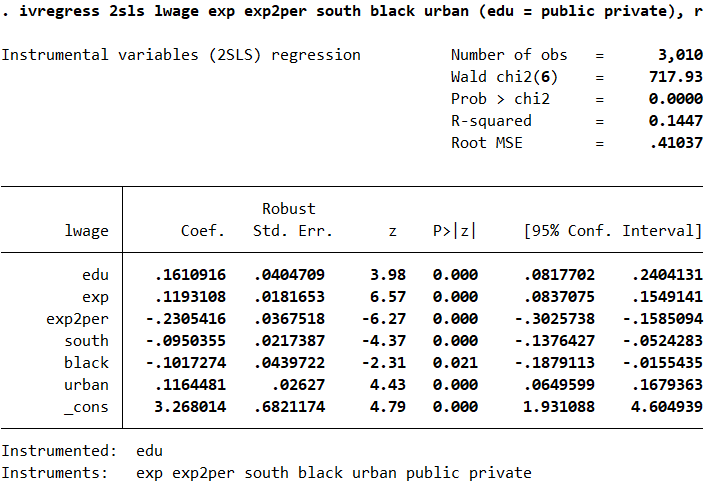
\includegraphics{p1}

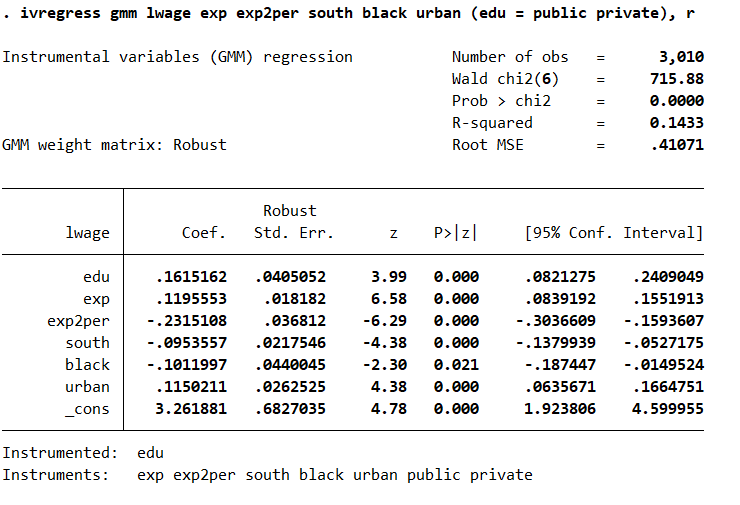
\includegraphics{p2}

The above outputs show almost no change from estimating the IV models via 2SLS vs GMM.

\subsection{Part B}
Output from the 2SLS and GMM outputs are below. Code for all parts will follow at the end of the question. 

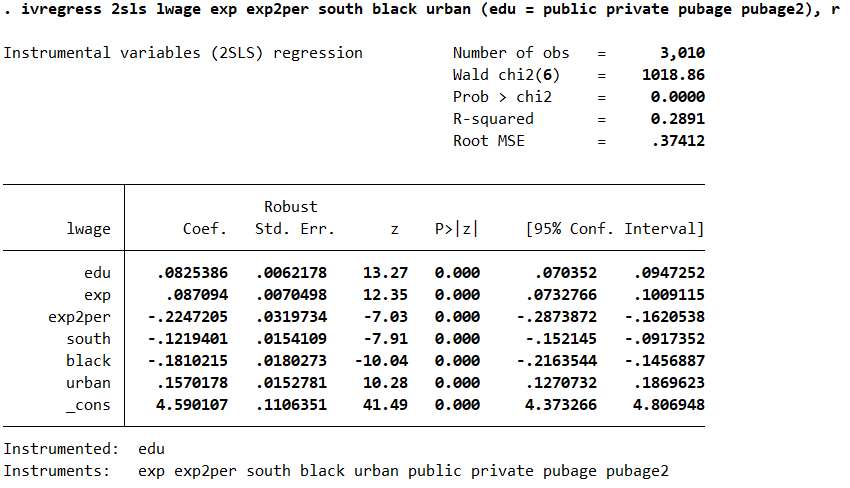
\includegraphics{p3}

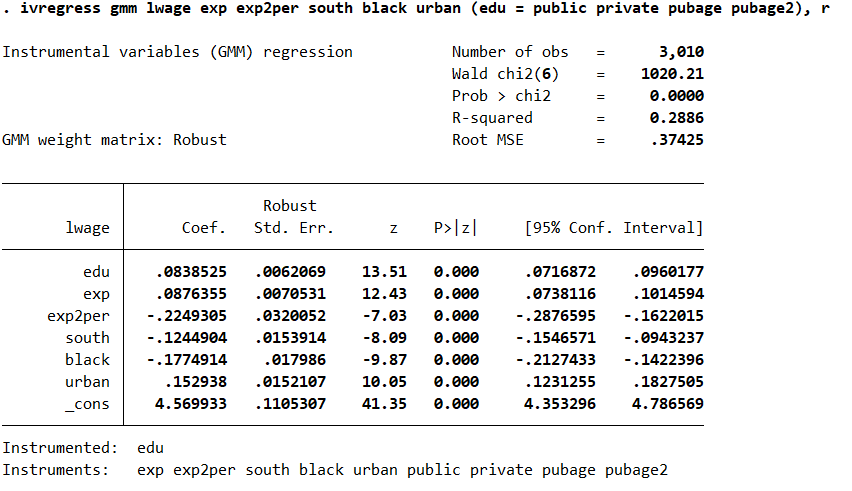
\includegraphics{p4}

As before, the above outputs show almost no change from estimating the IV models via 2SLS vs GMM.

\subsection{Part C}
Below, we report the J statistic for overidentification for both of the GMM models.

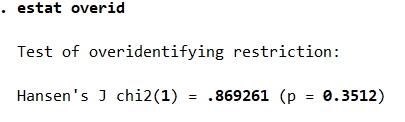
\includegraphics{p5}

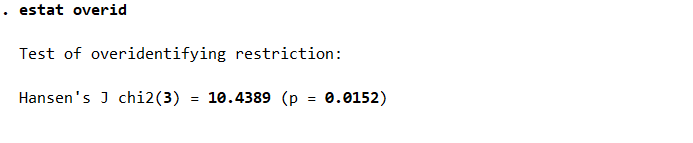
\includegraphics{p6}

Our J statistics show a major difference. The P value from the first model is quite large, while the P value from the second model is quite small, and significant at a 5 percent level. This may be caused by small sample distortions, but also may indicate that the model can be improved.

Below we display our code that generates the results presented above.

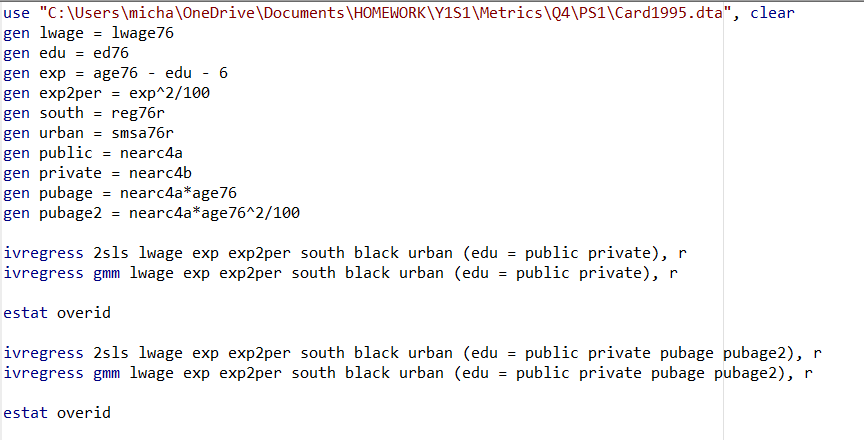
\includegraphics[scale=0.75]{p7}

\section{Question 17.15}

\subsection{Part A}
Output from the Arellano-Bond estimator is below. As in the previuous question, code for all parts will follow at the end of the question.

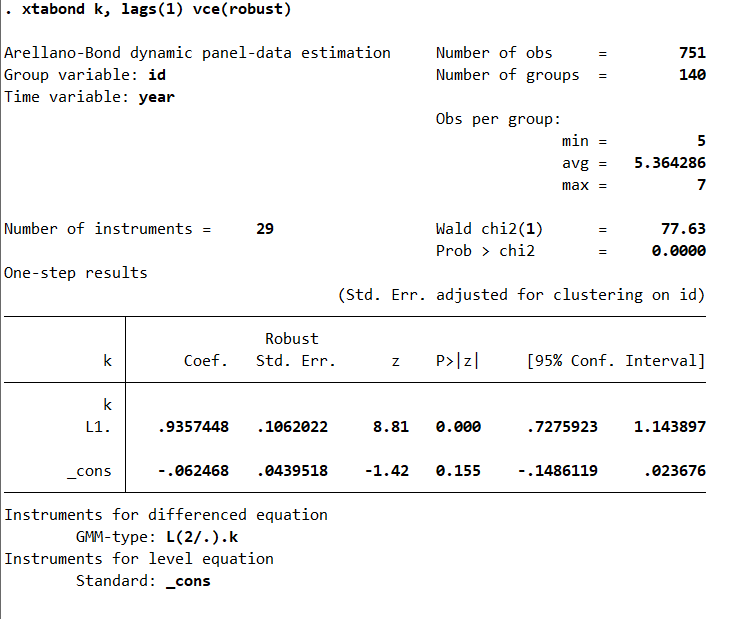
\includegraphics{p8}

\subsection{Part B}
Output from the Blundell-Bond estimator is below.

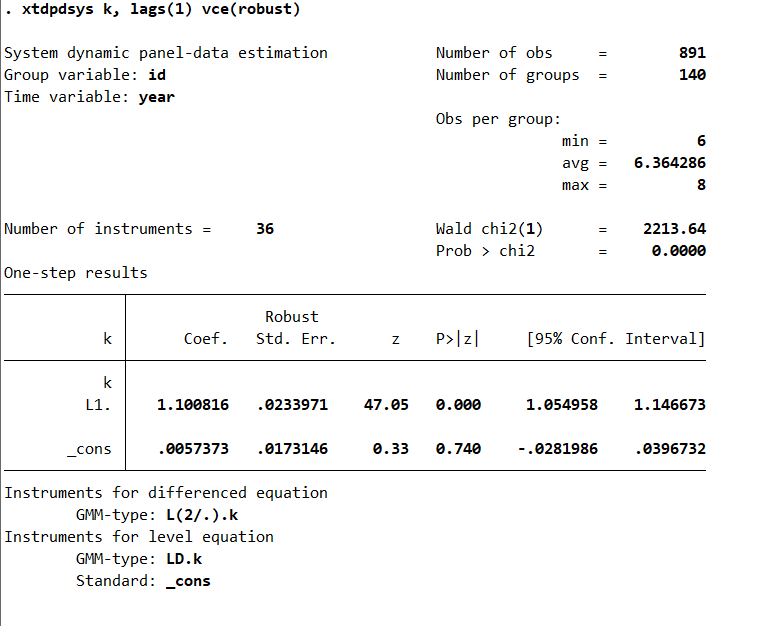
\includegraphics{p9}

\subsection{Part C}

Arellano-Bond suffers from a weak instrument problem if the true coefficient is near 1, i.e. if the true law of motion is close to a random walk. Our estimated coefficient from this model is in fact near 1, which means that this weak instrument issue seems to be a potential issue. As we saw in lecture, the Blundell-Bond estimator adds an extra assumption of stationarity, but avoids the weak instrument problem. In the results from the Blundell-Bond model, we see that the coefficient is again near 1. There are some differences between the results from the Blundell-Bond model and Arellano-Bond model. The differences are either due to (1) the weak instrument issue caused by the near-one lag coefficient, (2) the additional assumption of stationarity made by the Blundell-Bond model, which may or may not be true, or some combination of the two.

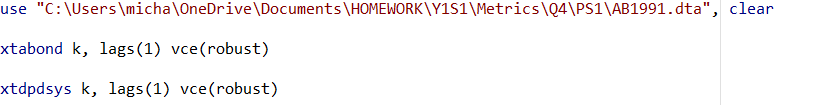
\includegraphics[scale=0.75]{p10}
\end{document}
